\documentclass{beamer}

\usetheme{default}
\usecolortheme{default}
\usefonttheme{default}

\title{Low-Level Network Programming and Operating Systems Development}
\author{Jacob Bates}
\institute{Da Vinci Science High School}

\begin{document}

\section{Title}

    \begin{frame}
        \titlepage
    \end{frame}

\section{Project}

    \begin{frame}{Project}
        The goal of this project was to implement a \textbf{network driver} and \textbf{network stack} at the \textbf{base level}.
        This was to be accomplished through writing an \textbf{operating system} for the \textbf{IA-32 Architecture} in the \textbf{C Programming Language}.
        The system was to be implemented as a \textbf{TFTP Storage Server}.\\
        \rule{0.5\textwidth}{0.5pt}\\
        I took on this project because I was already very involved with and interested in low-level programming, and I wanted to learn more specifically about networking.
    \end{frame}

\section{Hardware}

    \begin{frame}{Network Adaptor - Realtek RTL8139}
        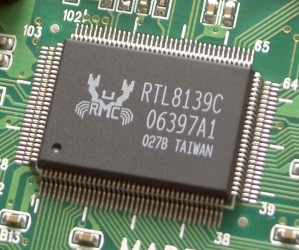
\includegraphics[height=125pt]{Realtek_RTL8139C.jpg} \\
        \rule{0.5\textwidth}{0.5pt} \\
        \begin{itemize}
            \item Widely Used on Older Machines
            \item Easier to Program
            \item Inexpensive
        \end{itemize}
    \end{frame}

\section{Protocols}

    \begin{frame}{Medium Access Control (MAC)}
        \begin{itemize}
            \item Data-Link-Layer Protocol
            \item Addresses Packets to a Machine
        \end{itemize}
    \end{frame}

    \begin{frame}{The Internet and The Internet Protocol}
        \begin{itemize}
            \item Network-Layer Protocol
            \item Addresses Packets to a Host
            \item Forwarded through Several Networks of Routers
        \end{itemize}
    \end{frame}

    \begin{frame}{The Internet Protocol Suite}
        \begin{block}{Internet Control Message Protocol (ICMP)}
            Used for Sending Essential Messages (e.g. Unreachable, Timestamp, PING)
        \end{block}

        \begin{block}{User Datagram Protocol (UDP)}
            \begin{itemize}
                \item Connectionless
                \item Datagram-Oriented
            \end{itemize}
        \end{block}

        \begin{block}{Transmission Control Protocol (TCP)}
            \begin{itemize}
                \item Connection-Oriented
                \item Provides a Stream of Data
            \end{itemize}
        \end{block}

        UDP and TCP are Transport-Layer Protocols, and Abstract Ports
    \end{frame}

\section{Implementation}

    \begin{frame}{Implementation - Network Adaptor}

    \end{frame}

    \begin{frame}{Implementation - Network Protocols}

    \end{frame}

\section{What I Learned}

    \begin{frame}{What I Learned}
        \begin{block}{Networking}
            Through this project, I gained a deep understanding of how the Computer Networks and the Internet work at the lowest level.
        \end{block}
        \begin{block}{System Architecture}
            In addition to what I've already learned about the X86 architecure, this project made me learn more about interrupts and the MMU.
        \end{block}
    \end{frame}

\end{document}
